\documentclass{beamer}
\usepackage[utf8]{inputenc}
\usepackage{multicol}
\usetheme{Madrid}
%\usecolortheme{wolverine}
\usecolortheme{default}
\setlength{\columnsep}{1cm}
%------------------------------------------------------------
%This block of code defines the information to appear in the
%Title page
\title[Phase 2: Erfassung und Auswertung] %optional
{Computer Vision zur bildbasierten Geodatenerfassung}

\subtitle{Projekt: Reconstruction of Landmarks}

\author[Projekt: Reconstruction of Landmarks] % (optional)
{ \Large\textbf{Phase 2: Erfassung und Auswertung der Bilder}
	\\[10mm]
	\small Yihan Tao\\
	Hsin-Feng Ho\\
	Jiaxin Liu}

%\institute[] % (optional)
%{
%\normalsize\textbf{Betreuer:} Dr. Michael Cramer\\
%Universität Stuttgart\\[3mm]
%}

\date[] % (optional)
{Stuttgart, November 2021}

\titlegraphic{\vspace{-10pt}\hspace{10cm}
\includegraphics[width=2cm]{ifp_logo}}

%--------------\vspace{-5cm}------------------------------
%The next block of commands puts the table of contents at the 
%beginning of each section and highlights the current section:

\AtBeginSection[]
{
	\begin{frame}
		\frametitle{Table of Contents}
		\tableofcontents[currentsection]
	\end{frame}
}
%------------------------------------------------------------


\begin{document}
	
	%The next statement creates the title page.
	\frame[plain]{\titlepage}
	
	
	%---------------------------------------------------------
	%This block of code is for the table of contents after
	%the title page
%	\begin{frame}
%		\frametitle{Table of Contents}
%		\tableofcontents
%	\end{frame}
	%---------------------------------------------------------
	
	
%	\section{Datensatz}
	
	%---------------------------------------------------------
	%Changing visivility of the text
	\begin{frame}\vspace{20pt}

		\frametitle{Kameraposition}
%		\textbf{Flight 1(low) + Flight 2 (high) combined}
		\vspace{-10pt}
		\begin{figure}[r]
		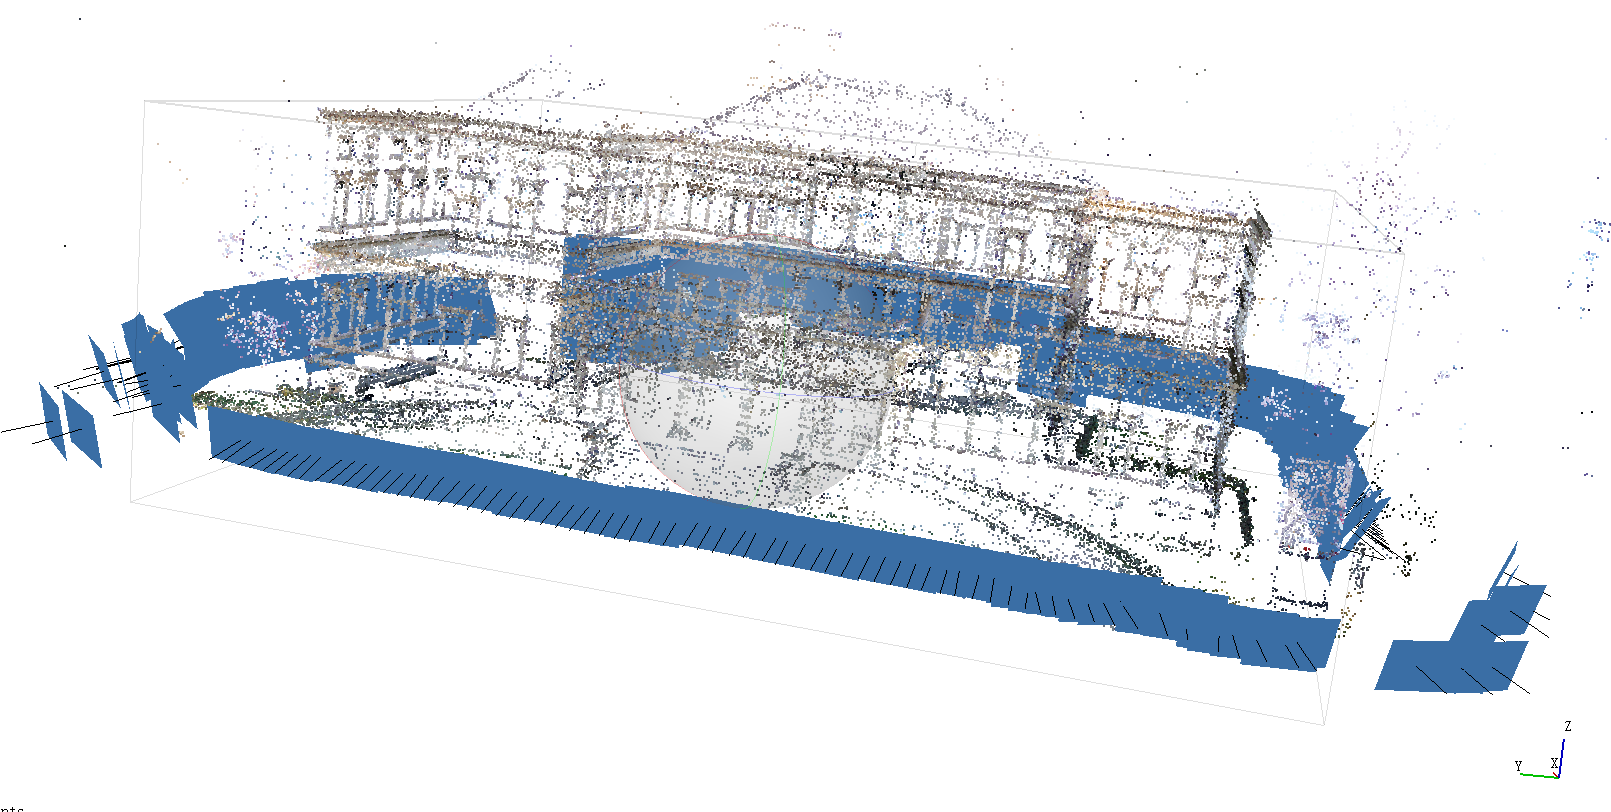
\includegraphics[width=12cm]{align photos}
%		\caption{dji Phantom 4 RTK Drohne}
		\end{figure}
%		\begin{itemize}
%			\item<1-> Text visible on slide 1
%			\item<2-> Text visible on slide 2
%			\item<3> Text visible on slides 3
%			\item<4-> Text visible on slide 4
%		\end{itemize}
	\end{frame}
	
	\begin{frame}
		\frametitle{Georeferencing}
		\begin{figure}[r]
			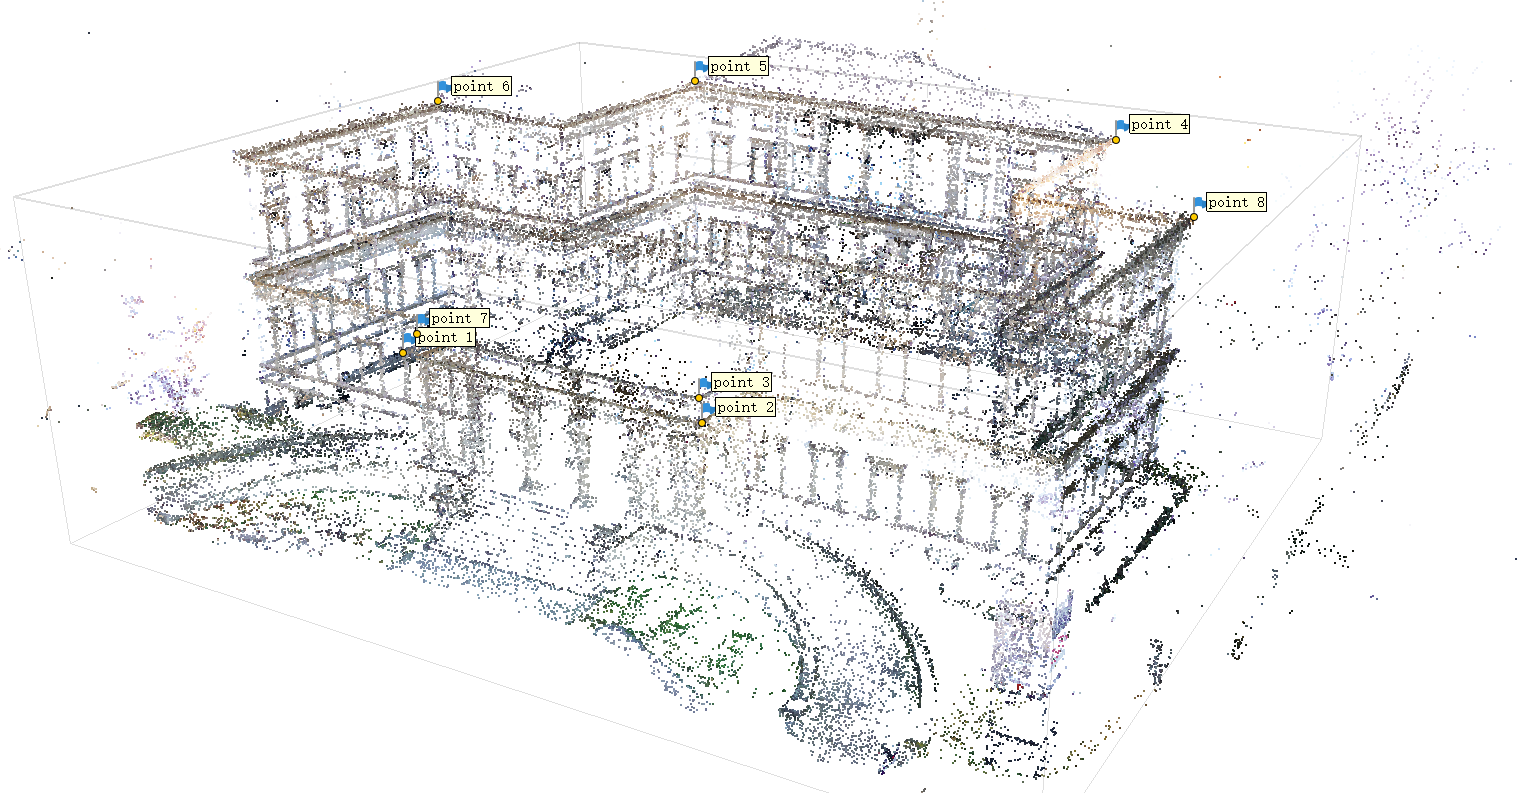
\includegraphics[width=12cm]{reference (GCPS)}
		\end{figure}	\end{frame}
		\begin{frame}
		\frametitle{Georeferencing}
		\begin{figure}[r]
			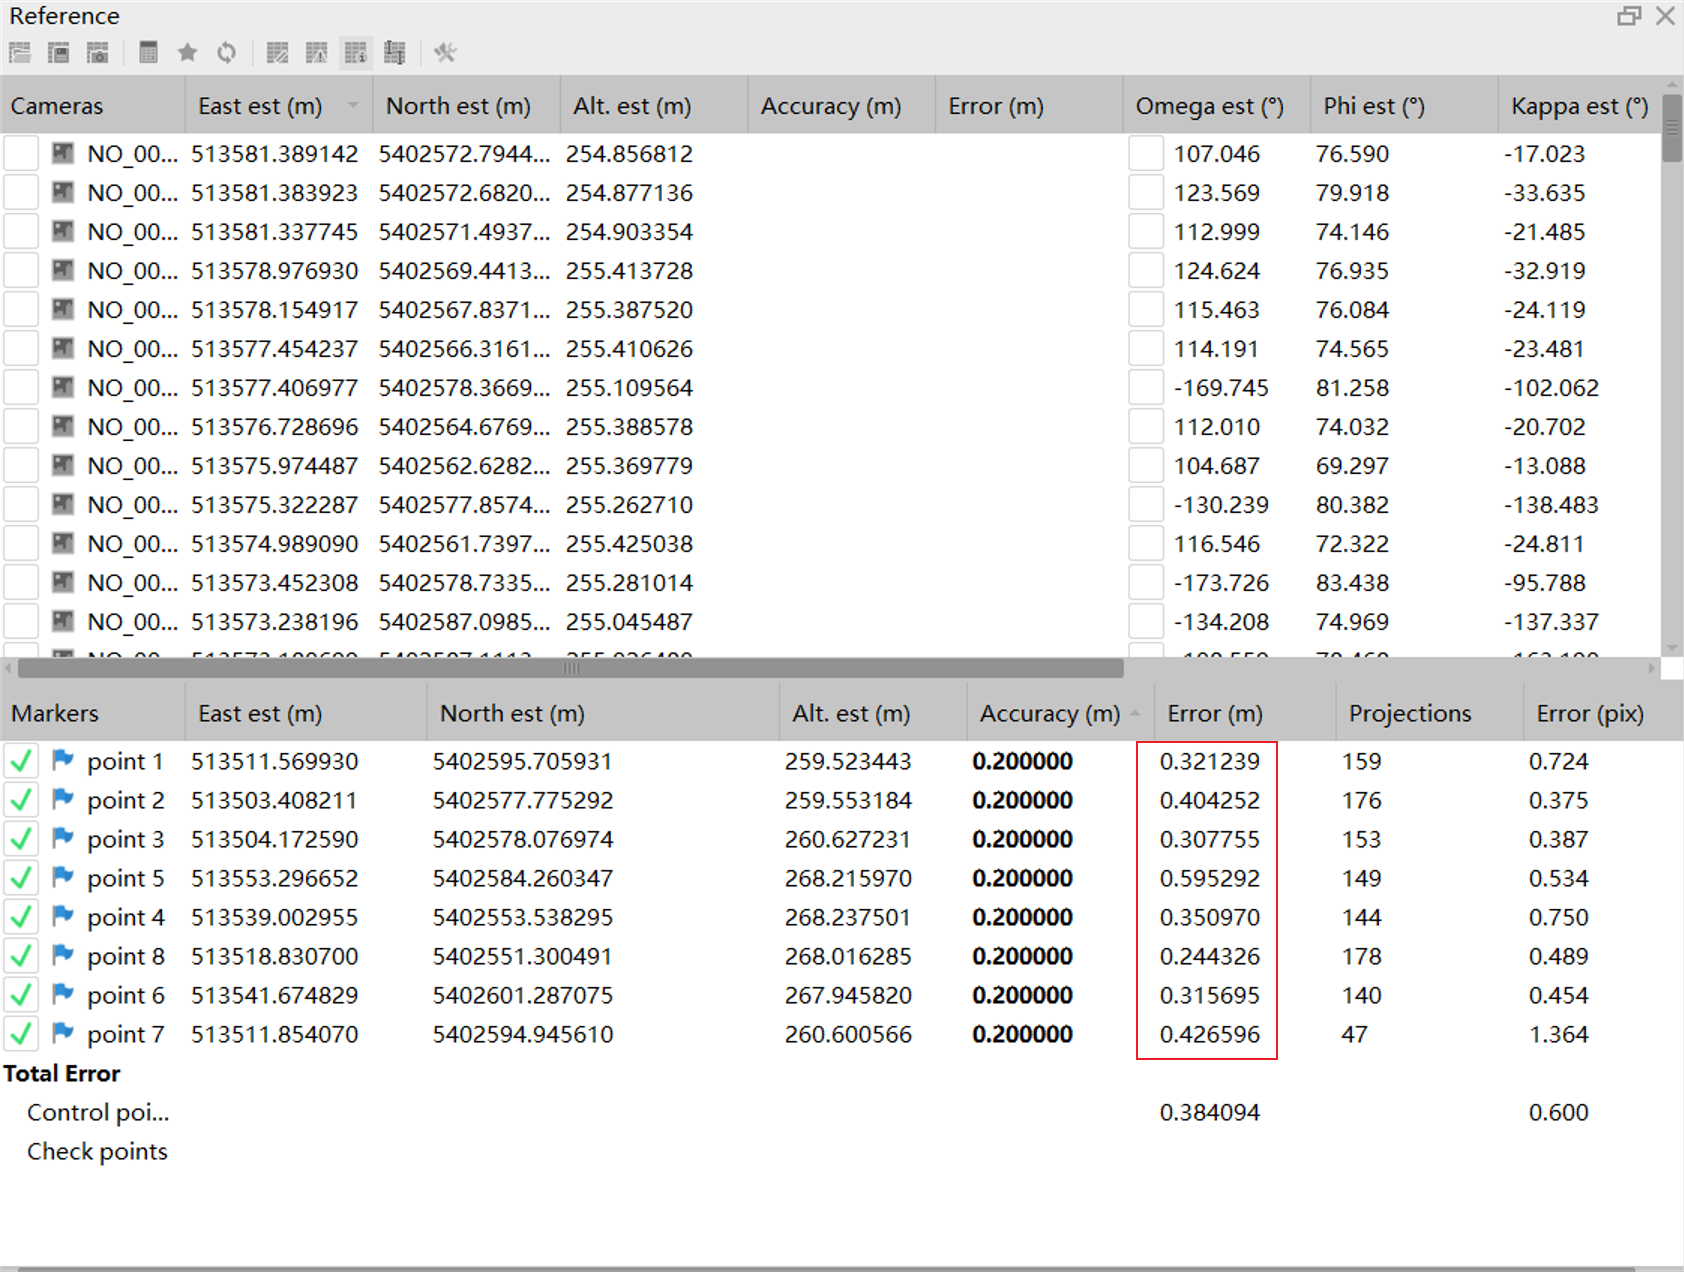
\includegraphics[width=10cm]{reference}
	\end{figure}	\end{frame}
\begin{frame}
\frametitle{Dense Cloud}
	\begin{figure}[r]
	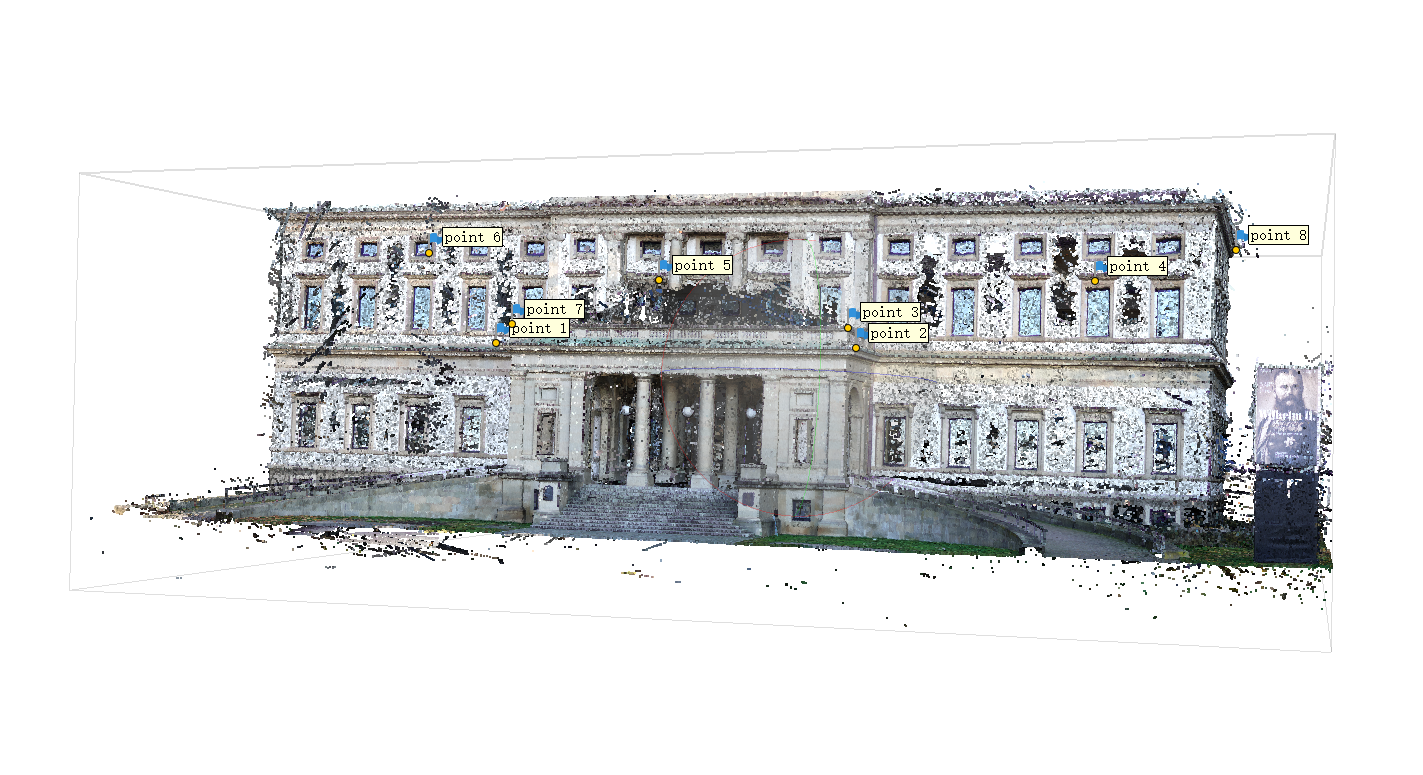
\includegraphics[width=12cm]{Dense Cloud 1}
\end{figure}\end{frame}

	\begin{frame}
	\frametitle{Scale}

	
	\begin{columns}
		
		\column{0.5\textwidth}
		\begin{figure}
			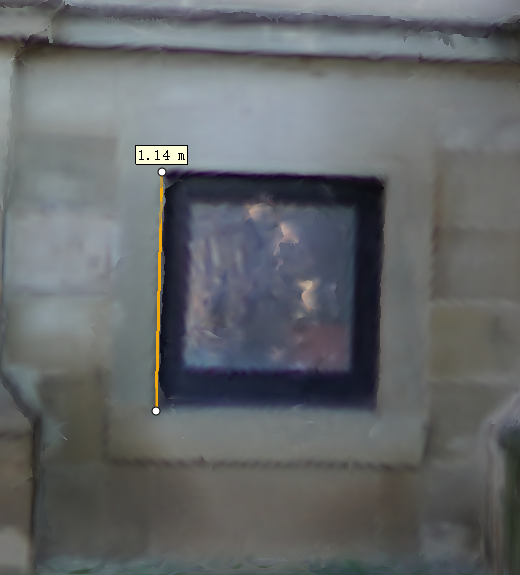
\includegraphics[scale=0.45]{Skale (In-Situ 1.14m)}
			\caption{1.14m in Realität}
		\end{figure}
		\column{0.5\textwidth}
		\vspace{20pt}
		\begin{figure}
			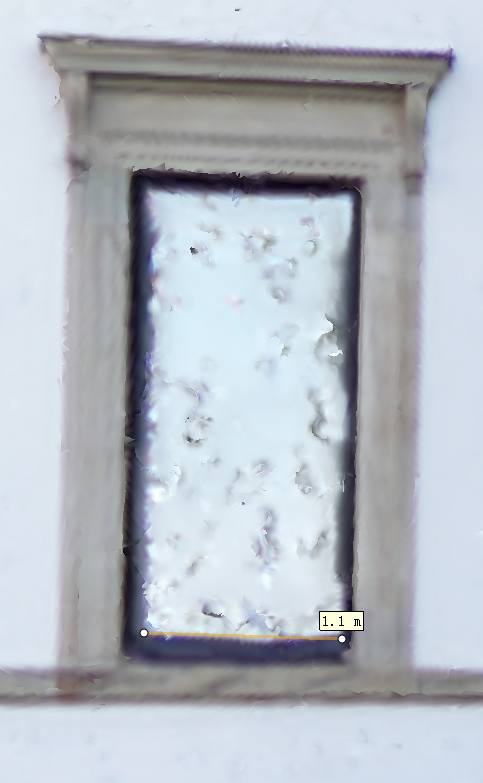
\includegraphics[scale=0.35]{Skale1(In-Situ 1.01 m)}
			\caption{1.01m in Realität}
		\end{figure}
		
	\end{columns}
\end{frame}

	\begin{frame}
		\frametitle{Mesh+Texture}
		\begin{figure}[r]
			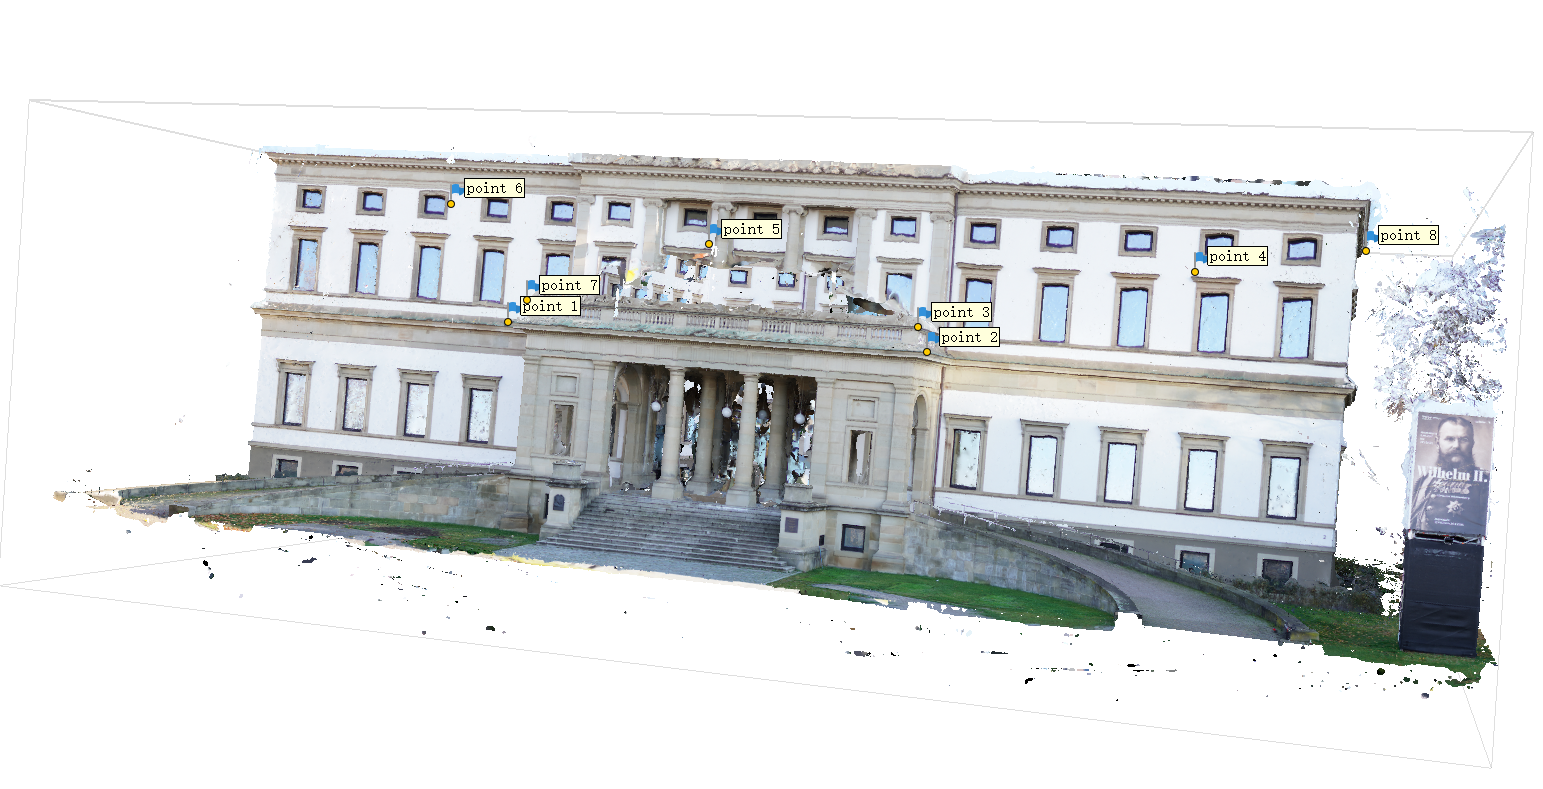
\includegraphics[width=12cm]{Mesh + Texture 1}
		\end{figure}
	\end{frame}

\end{document}